% Intestazione
\fancyhead[L]{3 \hspace{0.2cm} Processi di Supporto} % Testo a sinistra


\section{Processi di Supporto}


\subsection{Documentazione}
\label{sec:documentazione}

\subsubsection{Scopo}
Il \emph{processo}\textsubscript{\textit{\textbf{G}}} di documentazione mira a raccogliere le informazioni prodotte da un processo o
da un’attività nel \emph{ciclo di vita}\textsubscript{\textit{\textbf{G}}}, le decisioni prese dal gruppo e gli standard adottati per lo
svolgimento del progetto. È obbligatorio per tutti i membri del gruppo il rispetto di queste regole.

\subsubsection{Descrizione}
La documentazione costituisce una componente essenziale del progetto, poichè consente di
registrare ogni aspetto del lavoro svolto e delle decisioni prese. In particolare, questa sezione
raccoglie tutte le norme relative alla creazione, all’aggiornamento e al mantenimento della
documentazione (interna ed esterna) prodotta dal gruppo \emph{SWEg Labs} per ciascuna fase del
ciclo di vita del software.

\subsubsection{Aspettative}
Per quanto riguarda il processo di documentazione, il team ha le seguenti aspettative:
\begin{itemize}
    \item Definire delle procedure ripetibili che permettano di standardizzare il \emph{way of working}\textsubscript{\textit{\textbf{G}}}
    e la documentazione prodotta dal gruppo;
    \item Dichiarare le norme che i membri del gruppo sono tenuti a seguire per semplificare la
    redazione dei documenti.
\end{itemize}

\subsubsection{Ciclo di vita dei documenti}
Il ciclo di vita di ogni documento si compone delle seguenti fasi, visibili in Figura \bulref{fig:ciclo_vita_documentazione}:
\begin{itemize}
    \item \textbf{Redazione}:  documenti vengono scritti seguendo un approccio incrementale, e sono
    considerati redatti soltanto una volta completata la loro stesura;
    \item \textbf{Verifica}\textsubscript{\textit{\textbf{G}}}: ogni volta che i documenti vengono modificati necessitano di una verifica. 
    Ogni sezione coinvolta nella modifica di un documento viene verificata da una
    o più persone, chiamate verificatori. Il documento è considerato verificato una volta
    completate le verifiche da parte di tutti i verificatori incaricati;
    \item \textbf{Approvazione}: in questa fase, il Responsabile di Progetto dichiara che il documento
    è pronto per essere rilasciato, cioè che la sua stesura è completata ed è stato verificato.
    A questo punto, il documento viene marcato come approvato.
\end{itemize}

\begin{figure}[h]
    \centering
    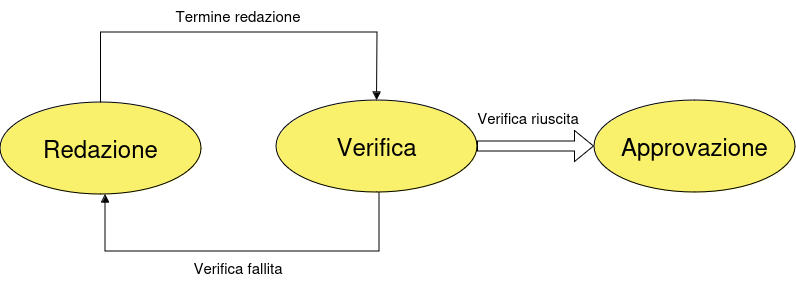
\includegraphics[width=0.6\textwidth]{Ciclo di vita della documentazione.png}
    \caption{Ciclo di vita della documentazione}
    \label{fig:ciclo_vita_documentazione}
\end{figure}


\subsubsection{Struttura dei documenti}
Ogni documento che verrà prodotto dovrà seguire una precisa struttura per garantire 
omogeneità e coesione.

\subsubsubsection{Numerazione di pagine}
La numerazione delle pagine del documento segue uno schema ben definito. Dalle pagine
iniziali e fino alla pagina precedente l’inizio del primo capitolo, viene utilizzata la numerazione
romana. Questa scelta mira a differenziare chiaramente la sezione introduttiva dal resto
del testo principale. Dopo questa fase preliminare, la numerazione prosegue con numeri
arabi, partendo da 1. Questo sistema offre una chiara progressione nel corpo principale del
lavoro. \\
Nel caso di appendici, la numerazione ritorna all’uso dei numeri romani, assegnando il numero 
I a ciascuna appendice.  Se ci sono più appendici, ogni volta che ne viene completata
una, si ricomincia la numerazione da I per la successiva. Questo approccio fornisce
un’organizzazione chiara e logica per le appendici, garantendo che ciascuna sia distintamente 
identificata. L’uso coerente di numeri romani e arabi in diverse sezioni del documento
contribuisce a una struttura ordinata e comprensibile per il lettore.

\subsubsubsection{Intestazione e piè di pagina}
In ciascuna pagina del documento, escludendo il frontespizio, sono presenti sia un’intestazione
che un piè di pagina. Nell’intestazione, sono inclusi i seguenti elementi:
\begin{itemize}
    \item Sul lato sinistro: il numero e il titolo del capitolo corrente;
    \item Sul lato destro: il logo del gruppo.
\end{itemize}
Nel piè di pagina, invece, sono indicati i seguenti dettagli:
\begin{itemize}
    \item Sul lato sinistro: il nome del file;
    \item Al centro: il numero della pagina attualmente in consultazione;
    \item Sul lato destro: il numero di versione del file.
\end{itemize}

\subsubsubsection{Frontespizio}
Il frontespizio, ovvero la prima pagina del documento,  strutturato nel seguente modo:
\begin{itemize}
    \item \textbf{Logo UniPD}: il logo universitario è posizionato in alto a sinistra;
    \item \textbf{Informazioni sul corso}: le informazioni relative al corso di Ingegneria del Software sono in alto a destra
    \item \textbf{Logo del gruppo}: il logo del gruppo è posizionato in alto a sinistra subito sotto al logo dell'Università;
    \item \textbf{Nome gruppo e recapito}: le informazioni sul gruppo \emph{SWEg Labs} sono posizionate in alto a destra, subito sotto alle info sul corso;
    \item \textbf{Titolo}: il titolo del documento è posizionato al centro della pagina, in grassetto;
    \item \textbf{Versione}: la versione del documento è posizionata al centro della pagina, appena sotto il titolo;
    \item \textbf{Tabella descrittiva}: posizionata centralmente sotto la versione del documento, riporta le seguenti informazioni:
    \begin{itemize}
        \item \textbf{Stato}: lo stato del documento nel suo ciclo di vita;
        \item \textbf{Redazione}: elenco dei membri del gruppo (nome e cognome) che hanno svolto la redazione del documento;
        \item \textbf{Verifica}: elenco dei membri del gruppo (nome e cognome) che hanno svolto la verifica del documento;
        \item \textbf{Approvazione}: elenco dei membri del gruppo (nome e cognome) che hanno svolto l’approvazione del documento;
        \item \textbf{Proprietario}: il proprietario del documento, nel nostro caso tutto il gruppo \emph{SWEg Labs};
        \item \textbf{Uso}: destinazione d’uso del documento (interno o esterno);
        \item \textbf{Destinatari}: destinatari del documento.
    \end{itemize}
\end{itemize}

\subsubsubsection{Registro delle modifiche}
Dopo la prima pagina si trova il registro delle modifiche. Tale registro va aggiornato ad ogni
modifica effettuata, specificando per ognuna:
\begin{itemize}
    \item \textbf{Versione}: la versione del documento in seguito alla modifica;
    \item \textbf{Data}: la data in cui è stata effettuata la modifica;
    \item \textbf{Descrizione}: una breve descrizione della modifica apportata;
    \item \textbf{Autore}: il nome e cognome dell’autore della modifica;
    \item \textbf{Verificatore}: il nome e cognome del verificatore della modifica, cioè
    colui che effettua la verifica del contenuto che è stato aggiungo, modificato o eliminato.
\end{itemize}

Le lettere di presentazione e i verbali, sia interni che esterni, non sono dotati del registro delle modifiche in quanto
in seguito alla prima redazione poi non sono soggetti a modifiche future.

\subsubsubsection{Indice}
Tutti i documenti (tranne le lettere di presentazione per ragione di brevità) devono contenere 
un indice, collocato nella pagina successiva al registro delle modifiche. L’indice è utile per 
agevolare la consultazione del documento, riportando per ogni titolo di sezione (e sottosezione) 
del contenuto effettivo del documento la sua pagina iniziale. Ciascuna delle pagine del contenuto 
è identificata da un numero progressivo, partendo da 1. In caso di sottosezioni si segue il formato:
\begin{center}
    \textbf{[numero sezione].[numero sottosezione]}
\end{center}
Lo stesso formato vale per qualsiasi livello di annidamento delle sottosezioni.

\subsubsubsection{Elenco delle figure}
Nella pagina successiva all’indice è presente l’elenco delle figure. Esso riporta, per ogni figura
che compare all’interno del documento, il suo titolo e la pagina in cui si trova. Come avviene
per le sezioni, ciascuna figura è identificata da un numero progressivo, partendo da 1.

\subsubsubsection{Elenco delle tabelle}
Nella pagina successiva a quelle dedicate all’elenco delle figure è presente l’elenco delle tabelle.
Esso riporta, per ogni tabella che compare all’interno del documento, il suo titolo e la pagina
in cui si trova. Come avviene per le sezioni e per l’elenco delle figure, ciascuna tabella è
identificata da un numero progressivo, partendo da 1.

\subsubsubsection{Contenuto}
Si tratta del contenuto effettivo del documento. Il contenuto deve essere suddiviso in sezioni
e sottosezioni, ciascuna con il suo titolo in grassetto e numerato secondo i criteri descritti in
precedenza.

\subsubsubsection{Verbali}
I verbali sono documenti che riportano le discussioni e le decisioni prese durante incontri.
I verbali devono contenere le seguenti sezioni:
\begin{itemize}
    \item \textbf{Informazioni generali}: contiene le informazioni riguardanti l’incontro, come la data, l’ora, il luogo e i partecipanti;
    \item \textbf{Ordine del giorno}: elenco degli argomenti che si era pianificato di trattare durante l’incontro;
    \item \textbf{Diario della riunione}: riassunto delle discussioni e delle azioni operate durante l’incontro;
    \item \textbf{Decisioni}: elenco delle decisioni prese durante l’incontro, ciascuna munita di codice identificativo per consentirne il tracciamento;
    \item \textbf{Todo}: elenco delle cose da fare emerse durante l'incontro, ciascuna collegata ad una o più decisioni. Ogni voce include un codice 
    identificativo per il tracciamento nel backlog, specifica la/e decisione/i di origine e il responsabile assegnato.
\end{itemize}


\subsubsection{Convenzioni}
In seguito vengono riportate tutte le convenzioni che i documenti devono rispettare.

\subsubsubsection{Nomi dei file}
Tutti i nomi dei file devono seguire la convenzione dello \emph{snake case}\textsubscript{\textit{\textbf{G}}}, 
cioè devono iniziare con una lettera minuscola e in caso di più parole ciascuna di esse deve essere separata tramite
il carattere di underscore ("\_"), tranne la data presente nei verbali, le cui parti devono essere separate da un trattino ("-"). Dopo il nome 
vero e proprio del file segue il numero della versione di quest’ultimo.

\subsubsubsection{Stile del testo}
Qui sono descritti tutti i diversi tipi di formattazione del testo usati nei documenti e i contesti
nei quali vengono impiegati:
\begin{itemize}
    \item \textbf{Grassetto}: viene utilizzato per evidenziare termini negli elenchi puntati e per i titoli
    delle sezioni;
    \item \textbf{Corsivo}: viene utilizzato per parole di particolare rilevanza all’interno del documento, 
    per indicare il nome del gruppo (\emph{SWEg Labs}), il nome dell’azienda \emph{proponente}\textsubscript{\textit{\textbf{G}}} 
    (\emph{AzzurroDigitale Srl}) e per le parole che si riferiscono al glossario (seguite da \textsubscript{\textit{\textbf{G}}});
    \item \textbf{Link}: i link sono i collegamenti ipertestuali, ovvero collegamenti a fonti esterne al
    documento. Essi sono mostrati sottolineati e in grassetto, mentre vengono evidenziati in giallo
    al momento del passaggio del cursore.
\end{itemize}

\subsubsubsection{Elenchi puntati}
Gli elenchi puntati sono utilizzati per gli elenchi oppure per esprimere concetti in modo più
diretto. Ciascuna voce di un elenco puntato è identificata da un simbolo, che varia a seconda
del livello di profondità in cui si trova. In particolare:
\begin{itemize}
    \item Un pallino per il primo livello;
    \begin{itemize}
        \item Un trattino per il secondo livello;
        \begin{itemize}
            \item Un asterisco per il terzo livello;
            \begin{itemize}
                \item Un punto per il quarto livello.
            \end{itemize}
        \end{itemize}
    \end{itemize}
\end{itemize}
Ogni voce inizia con la lettera maiuscola e termina con un punto e virgola (”;”), eccezione
fatta per l’ultima voce che termina con un punto (”.”).

\subsubsubsection{Formato delle date}
Per le date, viene adottato il seguente formato:
\begin{center}
    \textbf{DD/MM/YYYY}
\end{center}
dove:
\begin{itemize}
    \item \textbf{DD}: indica il giorno con 2 cifre;
    \item \textbf{MM}: indica il mese con 2 cifre;
    \item \textbf{YYYY}: indica l’anno con 4 cifre.
\end{itemize}

\subsubsubsection{Sigle}
Una lista di sigle presente all'interno dei documenti è la seguente:
\begin{itemize}
    \item \textbf{Ruoli}:
    \begin{itemize}
        \item \textbf{Re}: Responsabile di Progetto;
        \item \textbf{Am}: Amministratore di Progetto;
        \item \textbf{An}: Analista;
        \item \textbf{Pt}: Progettista;
        \item \textbf{Pr}: Programmatore;
        \item \textbf{Ve}: Verificatore.
    \end{itemize}
    \item \textbf{Revisioni di progetto}:
    \begin{itemize}
        \item \textbf{RTB}: \emph{Requirements and Technology Baseline}\textsubscript{\textit{\textbf{G}}};
        \item \textbf{PB}: \emph{Product Baseline}\textsubscript{\textit{\textbf{G}}}.
    \end{itemize}
\end{itemize}

\subsubsubsection{Tabelle}
Le tabelle di ogni documento devono rispettare le seguenti convenzioni:
\begin{itemize}
    \item Devono essere centrate orizzontalmente all’interno della pagina;
    \item Dopo ogni tabella segue una breve didascalia descrittiva accompagnata da un numero
    identificativo della stessa, incrementale e univoco all’interno del documento;
    \item Nelle celle che contengono solo uno 0 (zero), esso viene sostituito con un trattino per
    aumentarne la leggibilità.
\end{itemize}

\subsubsubsection{Immagini}
Ciascuna immagine, come le tabelle, deve essere centrata orizzontalmente all’interno della
pagina ed è seguita da una breve didascalia descrittiva comprensiva di un numero che le
identifica univocamente, incrementale all’interno del documento. Anche i grafici, 
\emph{diagrammi di Gantt}\textsubscript{\textit{\textbf{G}}} e \emph{diagrammi UML}\textsubscript{\textit{\textbf{G}}} 
sono inseriti nei documenti come immagini, pertanto seguono le stesse regole.


\subsubsection{Strumenti}
Per la redazione dei documenti, il gruppo \emph{SWEg Labs} ha scelto di utilizzare i seguenti strumenti:
\begin{itemize}
    \item \textbf{\emph{\LaTeX}}\textsubscript{\textit{\textbf{G}}}: per la redazione dei documenti il gruppo ha scelto il linguaggio \LaTeX. Si tratta
    di un linguaggio di markup basato su TeX per la produzione di documenti tecnici e scientifici di alta qualità;
    \item \textbf{\emph{Visual Studio Code}}\textsubscript{\textit{\textbf{G}}}: come editor di testo, il gruppo utilizza Visual Studio Code, 
    preferito per la sua leggerezza, versatilità e il supporto per estensioni personalizzabili;
    \item \textbf{\emph{GitHub}}\textsubscript{\textit{\textbf{G}}}: GitHub è utilizzato come piattaforma di versionamento e repository per la documentazione. 
    Consente una gestione collaborativa, permettendo il tracciamento delle modifiche e la revisione del testo in tempo reale;
    \item \textbf{\emph{draw.io}}\textsubscript{\textit{\textbf{G}}}: il team ha optato per Draw.io per disegnare i diagrammi UML necessari
    alla realizzazione del progetto didattico.
    \item \textbf{\emph{Fogli Google}}\textsubscript{\textit{\textbf{G}}}: i Fogli di calcolo di Google sono utilizzati dal team per creare e 
    aggiornare i grafici richiesti dal progetto.
\end{itemize}




\subsection{Gestione della configurazione}
\label{sec:gestione_configurazione}

\subsubsection{Scopo}
L’obiettivo di questa sezione è delineare l’approccio adottato dal gruppo \emph{SWEg Labs} nella 
gestione della configurazione, ossia la strategia scelta dal team per tenere traccia della
documentazione redatta e del codice sviluppato.

\subsubsection{Aspettative}
Per quanto riguarda la gestione della configurazione, il gruppo ha le seguenti aspettative:
\begin{itemize}
    \item Possibilità di tracciare tutte le modifiche apportate ai documenti o al codice;
    \item Possibilità di condivisione dei file tra i vari membri del gruppo;
    \item Possibilità di individuare e risolvere eventuali conflitti o errori;
    \item Possibilità di tornare ad una versione precedente.
\end{itemize}

\subsubsection{Descrizione}
L’obiettivo del processo di gestione della configurazione è garantire l’organizzazione e la
tracciabilità della documentazione e del codice, creando una storia per ogni file prodotto.
In particolare, si intende disporre i vari file all’interno di \emph{repository}\textsubscript{\textit{\textbf{G}}} 
facilmente accessibili e navigabili.


\subsubsection{Versionamento}

\subsubsubsection{Codice di versione}
Ad ogni modifica apportata ad un documento viene generata automaticamente una nuova
versione per quest’ultimo. Ogni versione è identificata dal suo codice, nel formato
\begin{center}
    \textbf{X.Y.Z}
\end{center}
dove:
\begin{itemize}
    \item \textbf{X}: rappresenta la versione dell’ultima approvazione da parte del responsabile;
    \item \textbf{Y}: rappresenta la versione dell’ultima approvazione generale da parte di un verificatore;
    \item \textbf{Z}: rappresenta la versione dell’ultima modifica, verificata da un verificatore.
\end{itemize}
Ogni approvazione comporta un incremento del numero di versione, che assume un peso
diverso a seconda della posizione della cifra incrementata: i cambiamenti più importanti
implicano un incremento della cifra più significativa.\\
Inoltre, un incremento ad una determinata cifra implica l’azzeramento di tutte le cifre alla
sua destra.

\subsubsubsection{Sistemi software utilizzati}
Per la gestione delle repository \emph{Git}\textsubscript{\textit{\textbf{G}}} si è deciso di utilizzare la 
piattaforma online \emph{GitHub}\textsubscript{\textit{\textbf{G}}}, in
quanto tutti i membri del gruppo hanno già familiarizzato in precedenza con questo sistema
software. Per quanto riguarda la gestione del \emph{backlog}\textsubscript{\textit{\textbf{G}}}, si è deciso di utilizzare
il servizio offerto da \emph{Jira}\textsubscript{\textit{\textbf{G}}}, dal momento che permette di usare strumenti avanzati per la
pianificazione, tracciamento e gestione dell’assegnazione delle varie attività.


\subsubsection{Struttura delle repository}
Con l’intento di organizzare al meglio il lavoro, si è optato per la creazione di due distinte 
repository pubbliche, al fine di mantenere separati i documenti organizzativi e il software:
\begin{itemize}
    \item \textbf{Documentazione}: per il versionamento della documentazione;
    \item \textbf{BuddyBot}: per il versionamento del codice.
\end{itemize}

\subsubsubsection{Documentazione}
All’interno di questa repository sono presenti le cartelle relative alle principali \emph{milestone}\textsubscript{\textit{\textbf{G}}}
del progetto, contenenti le rispettive \emph{baseline}\textsubscript{\textit{\textbf{G}}}:
\begin{itemize}
    \item \textbf{Candidatura}:  in questa cartella sono presenti i documenti prodotti per la candidatura
    d’appalto per il Capitolato C9. Il contenuto di questa cartella è il seguente:
    \begin{itemize}
        \item \textbf{Lettera di presentazione (v1.0.0)}: documento con cui il gruppo \emph{SWEg Labs} si
        candida formalmente per la realizzazione del progetto commissionato;
        \item \textbf{Preventivo dei costi e degli impegni orari (v1.0.0)}: documento che contiene 
        l’impegno orario per ciascun membro del gruppo, il costo totale preventivato per la
        realizzazione del progetto e la scadenza di consegna del prodotto software. Tali
        conclusioni sono tratte da alcune considerazioni preliminari sui ruoli che i membri
        del gruppo dovranno svolgere e da previa consultazione con il proponente \emph{AzzurroDigitale}\textsubscript{\textit{\textbf{G}}};
        \item \textbf{Valutazione dei Capitolati (v1.0.0)}: documento in cui il gruppo valuta 
        le criticità riscontrate per ogni capitolato d’appalto e motiva la scelta del
        capitolato selezionato;
        \item \textbf{Verbali}: cartella contenente tutti i verbali interni ed esterni (raccolti in apposite sottocartelle)
        relativi al periodo di candidatura;
    \end{itemize}
    \item \textbf{RTB}: in questa cartella sono presenti i documenti prodotti per la candidatura alla \emph{RTB}\textsubscript{\textit{\textbf{G}}}.
    Il contenuto è composto da:
    \begin{itemize}
        \item \textbf{\S\bulhref{https://sweg-labs.github.io/Documentazione/output/RTB/lettera_presentazione.pdf}{Lettera di Presentazione}};
        \item \textbf{Documentazione esterna}: sono contenuti i seguenti documenti:
        \begin{itemize}
            \item \textbf{\S\bulhref{https://sweg-labs.github.io/Documentazione/output/RTB/Documentazione\%20esterna/analisi_requisiti_v1.0.0.pdf}{Analisi dei Requisiti (v1.0.0)}};
            \item \textbf{\S\bulhref{https://sweg-labs.github.io/Documentazione/output/RTB/Documentazione\%20esterna/glossario_v1.0.0.pdf}{Glossario}};
            \item \textbf{\S\bulhref{hhttps://sweg-labs.github.io/Documentazione/output/RTB/Documentazione\%20esterna/piano_progetto_v1.0.0.pdf}{Piano di Progetto (v1.0.0)}};
            \item \textbf{\S\bulhref{https://sweg-labs.github.io/Documentazione/output/RTB/Documentazione\%20esterna/piano_qualifica_v1.0.0.pdf}{Piano di Qualifica(v1.0.0)}};
            \item \textbf{Verbali esterni}: cartella che raccoglie tutti i verbali esterni relativi al periodo RTB;
        \end{itemize}
        \item \textbf{Documentazione interna}: al suo interno sono contenuti:
        \begin{itemize}
            \item \textbf{\S\bulhref{https://sweg-labs.github.io/Documentazione/output/RTB/Documentazione\%20interna/norme_progetto_v1.0.0.pdf}{Norme di Progetto (v1.0.0)}};
            \item \textbf{Verbali interni}: cartella che raccoglie tutti i verbali interni relativi al periodo RTB;
        \end{itemize}
    \end{itemize}
\end{itemize}

\subsubsubsection{BuddyBot}
Questa repository contiene il codice sorgente relativo al \emph{Proof of Concept} del progetto e le
istruzioni per scaricarlo e testarlo in locale (\emph{README.md}).
Inoltre, è presente un file chiamato prompt\_engineering.txt dove sono riportati tutti i tentativi operati 
per raggiungere un miglioramento dell'efficacia informativa delle risposte di BuddyBot, 
tra cui varie domande poste al chatbot e le corrispondenti risposte ottenute nel corso del tempo.

\subsubsubsection{Gestione delle modifiche}
Una buona suddivisione del lavoro tra i diversi documenti da redigere e le varie \emph{feature}\textsubscript{\textit{\textbf{G}}}
da sviluppare contribuisce significativamente a ridurre i conflitti. L’obiettivo è mantenere 
il \emph{branch}\textsubscript{\textit{\textbf{G}}} principale (\emph{main}) privo di errori, rendendolo inaccessibile a qualsiasi membro 
del gruppo fino all’approvazione del Responsabile di Progetto. Solo in seguito di tale
approvazione è consentito effettuare il \emph{merge}\textsubscript{\textit{\textbf{G}}} di uno dei rami minori nel \emph{main}.


\subsection{Gestione della Qualità}
\label{sec:gestione della qualità}

\subsubsection{Scopo}
Questa sezione ha l'obbiettivo di descrivere le modalità con cui il gruppo intende misurare la qualità dei processi e del prodotto finale, al fine di soddisfare le aspettative del proponente.

\subsubsection{Descrizione}
Il processo di gestione della qualità stabilisce le norme e gli strumenti per misurare della qualità dei processi e del prodotto finale. Sono specificati gli obbiettivi prefissati, i metodi per raggiungerli e per verificarne il compimento.

\subsubsection{Aspettative}
\begin{itemize}
    \item Soddisfare i requisiti di qualità richiesti dal proponente;
    \item Migliorare la qualità dei processi svolti dal gruppo;
    \item Valutare lo stato di avanzamento del progetto.
\end{itemize}

\subsubsection{Piano di Qualifica}
Per stabilire gli obbiettivi di questo processo utilizziamo il Piano di Qualifica. Ossia un documento contenente:
\begin{itemize}
    \item Gli obbiettivi qualitativi da raggiungere;
    \item Le definizioni e descrizioni delle metriche utilizzate per la misurazione della qualità dei processi, del prodotto, della documentazione e dei software utilizzati;
    \item La descrizione dei test da svolgere e le relative norme da seguire;
    \item Lo stato attuale della qualità del progetto, misurato tramite le metriche descritte.
\end{itemize}

\subsubsection{Strumenti}
Gli strumenti utilizzati per la gestione della qualità sono le metriche.
Queste sono le norme che regolano le metriche adottate, le quali rappresentano ognuna un conseguente obiettivo prefissato.
Le metriche adottate sono presentate e descritte nel documento piano di qualifica, ognuna con i seguenti parametri:
\begin{itemize}
    \item \textbf{Nome}: il nome della metrica
    \item \textbf{Codice}: ogni metrica ha un codice identificativo formato da:
    \begin{center}
        M[Tipologia][Id numerico]
    \end{center}
    dove
    \begin{itemize}
        \item \textbf{Tipologia} può essere:
        \begin{itemize}
            \item \textbf{PC} per processo;
            \item \textbf{PD} per prodotto.
        \end{itemize}
        \item \textbf{Id numerico} indica un numero univoco incrementale separato per le due tipologie.
    \end{itemize}
    \item \textbf{Processo}: indica a che processo fa riferimento la metrica;
    \item \textbf{Formula}: come la metrica viene matematicamente calcolata (opzionale);
    \item \textbf{Descrizione}: spiegazione di cosa rappresenta la metrica e di come valutarla e interpretarla;
    \item \textbf{Valore di accettabilità}: indica il valore della metrica considerato accettabile;
    \item \textbf{Valore di preferibilità}: indica il valore ideale che dovrebbe essere assunto.
\end{itemize}


\subsection{Verifica}
\label{sec:verifica}

\subsubsection{Scopo}
Questa sezione si propone di illustrare come il gruppo ha pianificato e implementato il processo di \emph{verifica}\textsubscript{\textit{\textbf{G}}}, finalizzato a valutare il prodotto software. Tale processo è essenziale per garantire che il software soddisfi i requisiti definiti e rispetti le aspettative. 

\subsubsection{Aspettative}
\begin{itemize}
    \item Garantire l'ottenimento del prodotto finale in linea con le aspettative;
    \item Individuare tempestivamente eventuali errori, riducendo sprechi di risorse e tempo;
    \item Consentire al gruppo di progredire nello sviluppo in maniera più sicura e accurata.
\end{itemize}

\subsubsection{Descrizione}
Il processo di \emph{verifica}\textsubscript{\textit{\textbf{G}}} si basa su \emph{test}\textsubscript{\textit{\textbf{G}}} e analisi per individuare e correggere eventuali errori emersi durante lo sviluppo del software o la redazione della documentazione, assicurando la conformità ai requisiti. Per una verifica efficace, è fondamentale applicare procedure definite, criteri affidabili e una sequenza di fasi che preparino al passaggio successivo, ossia la validazione. Di seguito sono illustrate le principali attività svolte in questo processo.

\subsubsection{\emph{Analisi statica}\textsubscript{\textit{\textbf{G}}}}
L’\emph{analisi statica} prende il nome dal fatto che non richiede l’esecuzione del codice e si presta anche all’applicazione sulla documentazione. Questa attività consiste in una revisione dettagliata del codice e dei documenti per assicurarsi che rispettino i vincoli stabiliti, siano privi di difetti e soddisfino le caratteristiche richieste
Il successo di questa analisi dipende in modo significativo dalla competenza e dall’attenzione dei verificatori coinvolti.

\subsubsection{\emph{Analisi dinamica}\textsubscript{\textit{\textbf{G}}}}
L'\emph{analisi dinamica} comprende tecniche che richiedono l'esecuzione del codice da verificare, rendendola applicabile esclusivamente al software, e non alla documentazione. 
Questa attività prevede l'esecuzione di \emph{test}\textsubscript{\textit{G}} per verificare il corretto funzionamento del software e identificare eventuali discrepanze tra i risultati attesi e quelli effettivi. Questo processo deve essere automatizzato e ripetibile. 
Per garantire l'efficacia dei test, ciascuno di essi deve essere deterministico, cioè, dati gli stessi input, deve produrre sempre lo stesso output. 
Inoltre, ogni test deve avere parametri ben definiti, tra cui:
\begin{itemize}
    \item descrizione dei parametri di input;
    \item descrizione dell'output;
    \item comportamento atteso del software;
    \item condizioni di esecuzione del test.
\end{itemize}
Al fine di agevolare l’automazione dei test, saranno utilizzati i seguenti strumenti:
\begin{itemize}
    \item \textbf{Driver:} una componente che fornisce l’ambiente di esecuzione necessario per testare un componente del prodotto software. Un driver è progettato per “attivare” il componente da testare e fornirgli i dati di input necessari;
    \item \textbf{Stub:} una componente passiva che simula il comportamento di alcune parti mancanti o non ancora implementate nell’applicazione. Questo consente di testare in anticipo le parti del software che dipendono da altre parti non ancora disponibili;
    \item \textbf{Logger:} uno strumento che registra i risultati ottenuti durante l’esecuzione del test, consentendo un’analisi accurata dei dati prodotti.
\end{itemize}

\subsubsection{Test di sistema}
I \emph{Test di sistema}\textsubscript{\textit{\textbf{G}}} hanno l’obiettivo di misurare la copertura dei requisiti specificati nel
capitolato d’appalto. Essi sono definiti durante l’\emph{Analisi dei Requisiti} e vengono svolti dopo
i \emph{test di integrazione}, dunque quando tutte le componenti del sistema software sono state
integrate. Questo tipo di test è svolto anche durante il processo di validazione.

\subsubsection{Test di accettazione}
I \emph{Test di accettazione}\textsubscript{\textit{\textbf{G}}} servono per dimostrare che i requisiti individuati sono stati
soddisfatti. Questo tipo di test deve essere svolto obbligatoriamente alla presenza del \emph{committente}.

\subsubsection{Codici relativi ai test}
Il gruppo ha deciso di classificare i \emph{test} che andranno svolti nell’attività di verifica associando un codice identificativo a ciascuno di essi nel formato
\begin{center}
    \textbf{T[tipo][codice]}
\end{center}T[tipo][codice]
dove:
\begin{itemize}
    \item \textbf{[tipo]} rappresenta il tipo di test, in particolare:
    \begin{itemize}
        \item S per i test di sistema;
        \item A per i test di accettazione.
    \end{itemize}
    \item \textbf{[codice]} è un numero progressivo associato al test all’interno del suo tipo.
\end{itemize}

%Ancora da capire se serve: Se il test in questione ha un padre, si segue il formato [codice padre].[codice figlio]
%dove [codice figlio] è un numero progressivo che identifica univocamente un test figlio del test con codice pari a [codice padre].

\subsubsection{Stato dei test}
Ad ogni test verrà associato uno stato che ne rappresenterà l’esito.
Lo stato può essere:
\begin{itemize}
    \item N-I: il test non è ancora stato implementato;
    \item Superato: il test riporta esito positivo;
    \item Non superato: il test riporta esito negativo.
\end{itemize}

\subsection{Validazione}
\label{sec:validazione}
\subsubsection{Scopo}
Questa sezione contiene le norme atte a regolare il processo di validazione, al fine di garantirne l'efficacia. Il processo di validazione permette di confermare l'effettivo conseguimento delle aspettative specificate dal proponente.
\subsubsection{Aspettative}
Tramite il processo di validazione il gruppo intende assicurarsi la conformità del prodotto software rispetto ai requisiti specificati nel documento di Analisi dei Requisiti.
\subsubsection{Descrizione}
La validazione si articola in più attività:
\begin{itemize}
    \item \textbf{Istanziazione delle procedure}: vengono stabilite le procedure e le strategie da attuare per garantire una validazione efficace;
    \item \textbf{Istanziazione tei test di accettazione}: un test di accettazione consiste in una serie di operazioni eseguite sul prodotto software finale che rispondono positivamente solo se il software soddisfa tutti i requisiti specificati, garantendo che sia conforme alle aspettative del proponente. Tali test devono essere riportati nel documento \emph{Piano di qualifica};
    \item \textbf{Collaudo}: i test di accettazione vengono effettuati sul prodotto software in presenza del proponente, ma non prima di aver svolto con successo i test di sistema in un ambiente identico a quello di installazione.
\end{itemize}
